Once we performed our case study and determined the metrics that might better represent the testability of the projects, in this section we resort to describe the results in detail using the metrics defined in the previous section.

After running the experiment over the 86, we detected 20 projects in which not a single test was run on any commit in the history. 
The learning-spark project does not contain any tests in any commit of its history. 
The Mycat-Server project has a dependency on software that must be installed on the machine for it to be compiled (therefore its Source Compilability is 0\%). 
The Clojure project is a programming language and as such, its tests require a different execution method. 
The remaining 17 projects correspond to projects that contain multiple Maven modules and cannot be compiled and tested with the proposed methodology. In general, when the multimodule parent project has the proper configuration, we are able to compile and run the tests from the parent module, which is from where we run the Maven command. However, in some cases, this approach does not work, and compiling and running tests would require knowing in which order modules need to be compiled so that tests for that or another module can be compiled and run. This is due to dependencies among modules that forces some modules to be built before others. 
%Despite the interest and the percentage of the total that these projects represent, we consider that they should be studied in a separate study.
Since we cannot execute any of the tests on any of these projects, we have decided to leave them out of our study, and from this point on we will only consider the remaining 66 projects.

% \begin{figure}[h!]
%     \centering    
%     \begin{tikzpicture}[node distance=1cm,every node/.style={fill=white, font=\sffamily}, align=center]
    \footnotesize
    % Specification of nodes (position, etc.)
    \node (total)             [large]                                         { 407,579 Commits};
    \node (buildable)         [large, below of=total]                         { 103,097 Source buildables commmits};
    \node (testBuildable)     [large, below of=buildable]                     { 93,925 Test buildables commits};
    \node (success)           [large, below of=testBuildable]                 { 40,540 Testable commits};

    \draw[-Latex]             (total) -- (buildable);
    \draw[-Latex]             (buildable) -- (testBuildable);
    \draw[-Latex]             (testBuildable) -- (success);

\end{tikzpicture}
%     \caption{Study overview 
%     \label{fig:methodology-process}
% \end{figure}

Table~\ref{table:results-1} shows a summary of the experiment for the 66 projects. 
In the \textit{Count} column we can see the magnitude of the study for the metrics defined in the methodology. 
The Mean ({\large$\mean{x}$}) and Median ({\large$\median{x}$}) columns show the trend at the project level.
We run a normality test for each metric in this table, finding that with the exception of \textit{Age}, none of the metrics shows a normal distribution. 
In general, differences between mean and median show large internal variability in each of the samples.

\begin{table}[!htb]
    \centering
    \caption{Absolute results.}
    \label{table:results-1}
    \begin{tabular}{|r|r|r|r|}
        \hline
        \multicolumn{1}{|c|}{\textbf{Metric}}& \multicolumn{1}{c|}{\textbf{Count}} & \multicolumn{1}{c|}{\textbf{\large{$\mean{x}$}}} & \multicolumn{1}{c|}{\textbf{\large{$\median{x}$}}} \\ \hline
        \textbf{Age}                      & 634.66                              & 9.62                               & 9.69                                 \\ \hline
        \textbf{LoC}                      & 11,143,058                         & 174,110.28                          & 26,973.50                             \\ \hline
        \textbf{Commits}                  & 407,579                           & 6,175.44                            & 2,831.00                              \\ \hline
        \textbf{Source-compilable commits} & 103,097                           & 1,562.08                            & 1,020.00                              \\ \hline
        \textbf{Test-compilable commit}    & 93,925                            & 1,423.11                            & 692.50                               \\ \hline
        \textbf{Fully Testable commits}   & 40,540                            & 614.24                             & 218.00                               \\ \hline
    \end{tabular}
\end{table}

Table~\ref{table:results-3} shows information on the compilability and testability metrics of the projects of the dataset.

\begin{table}[h]
    \centering
    \caption{Mean ($\mean{x}$) and Median ($\median{x}$) values for Compilability and Testability of the projects.}
        \label{table:results-3}
        \begin{tabular}{|r|r|r|}
            \hline
            \multicolumn{1}{|c|}{\textbf{Metric}} & \multicolumn{1}{c|}{\textbf{Mean}} & \multicolumn{1}{c|}{\textbf{Median}} \\ \hline
            \textbf{Source Compilability}                         & 47.29\%                              & 47.12\%                                \\ \hline
            \textbf{Test Compilability\textsubscript{A}}          & 41.73\%                              & 39.22\%                                \\ \hline
            \textbf{Test Compilability\textsubscript{S}}          & 88.26\%                              & 97.35\%                                \\ \hline
            \textbf{Testability Rate\textsubscript{A}}           & 38.63\%                              & 34.88\%                                \\ \hline
            \textbf{Testability Rate\textsubscript{T}}           & 94.14\%                              & 99.53\%                                \\ \hline
            \textbf{Fully Testability\textsubscript{A}}          & 22.12\%                              & 14.88\%                                \\ \hline
            \textbf{Fully Testability\textsubscript{T}}          & 52.53\%                              & 59.32\%                                \\ \hline
    \end{tabular}
\end{table}


To illustrate the diversity of the results, we have divided the 66 projects into three groups of the same size according to their number of commits: large, medium and small. 
Figures~\ref{fig:many4j-1-bar-chart} (large projects), \ref{fig:many4j-2-bar-chart} (medium projects) and \ref{fig:many4j-3-bar-chart} (short projects) show the results for each project for each of the integer metrics as overlapping bars.
% To illustrate the diversity of results across the projects, we have represented the different categories of commits per project in overlapped bars in Figures~\ref{fig:many4j-1-bar-chart} (large projects), \ref{fig:many4j-2-bar-chart} (medium projects) and \ref{fig:many4j-3-bar-chart} (short projects).
% The division of projects into the three categories (long, medium and short) is based on the number of commits.
It is easy to appreciate, just by checking colors, how each project tells a very different story. 

\begin{figure}[h!]
    \centering    
    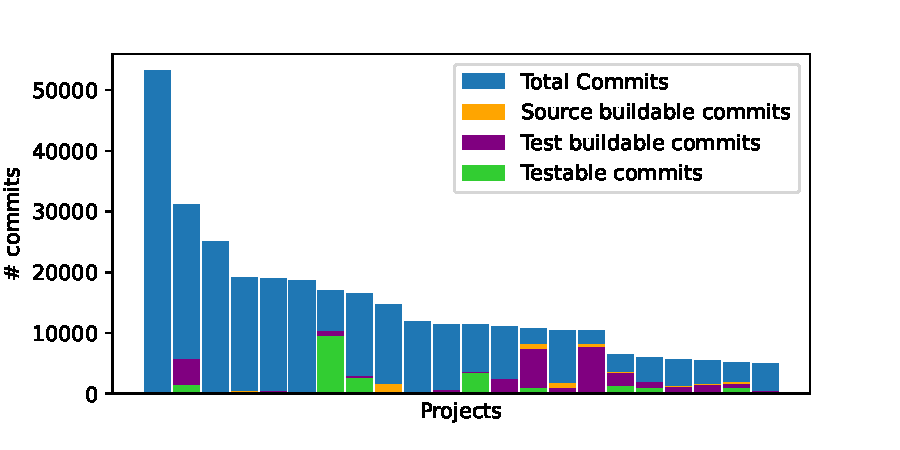
\includegraphics[width=0.8\textwidth]{pages/02-Testability/images/Many4j 1-22.pdf}
    \caption{Project metrics (Large projects)}
    \label{fig:many4j-1-bar-chart}
\end{figure}%
\begin{figure}[h!]
    \centering    
    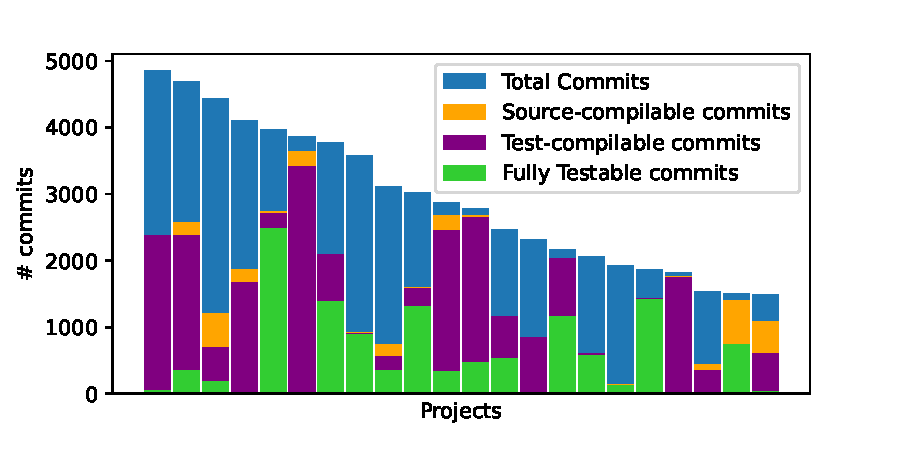
\includegraphics[width=0.8\textwidth]{pages/02-Testability/images/Many4j 23-44.pdf}
    \caption{Project metrics (Medium projects)}
    \label{fig:many4j-2-bar-chart}
\end{figure} 
\begin{figure}[h!]
    \centering    
    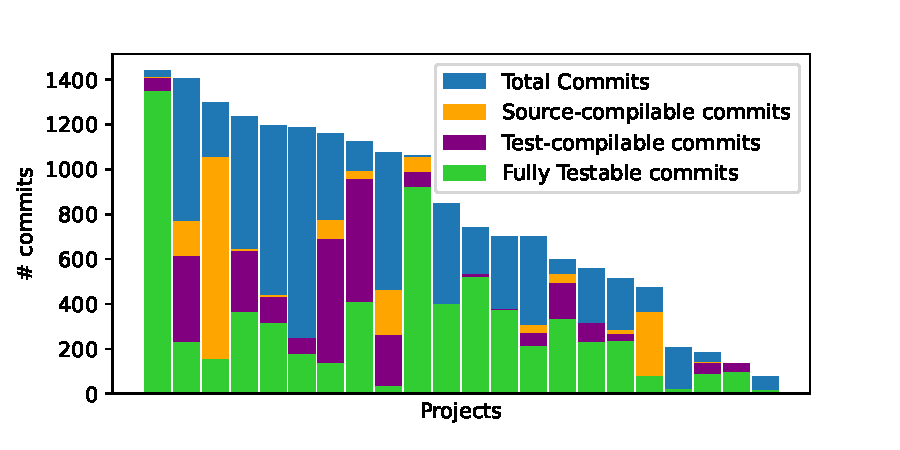
\includegraphics[width=0.8\textwidth]{pages/02-Testability/images/Many4j 45-66.pdf}
    \caption{Project metrics (Short projects)}
    \label{fig:many4j-3-bar-chart}
\end{figure}

\newpage